A parameter sweep was performed using LULESH, described in Section
\ref{sec:lulesh}. The device clock was varied from 500MHz to 1312MHz to 1800MHz.
The memory clock was varied from 877MHz to 1200MHz to 1600MHz. Figure
\ref{fig:lulesh_sweep} shows the results, where lower runtime time is better.


As expected, changing the frequency of the backing store has little effect on
LULESH for this problem size because it is not memory bandwidth bound. The most
improvement is seen at the low device clock frequency, but at this frequency
the speedup is still small at 1.04x.
However, increasing the frequency of the SMs does improve the
performance noticeably. Going from 500MHz to 1312MHz shows a 2.5x speedup; going
from 1312MHz to 1800MHz shows a further 1.3x speedup.

Although this was a small study, one can imagine being able to run a more
complete parameter sweep over any of the Balar parameters.

   \begin{figure}[!htb]
      \centering
      \setlength{\abovecaptionskip}{6pt plus 1pt minus 1pt}
      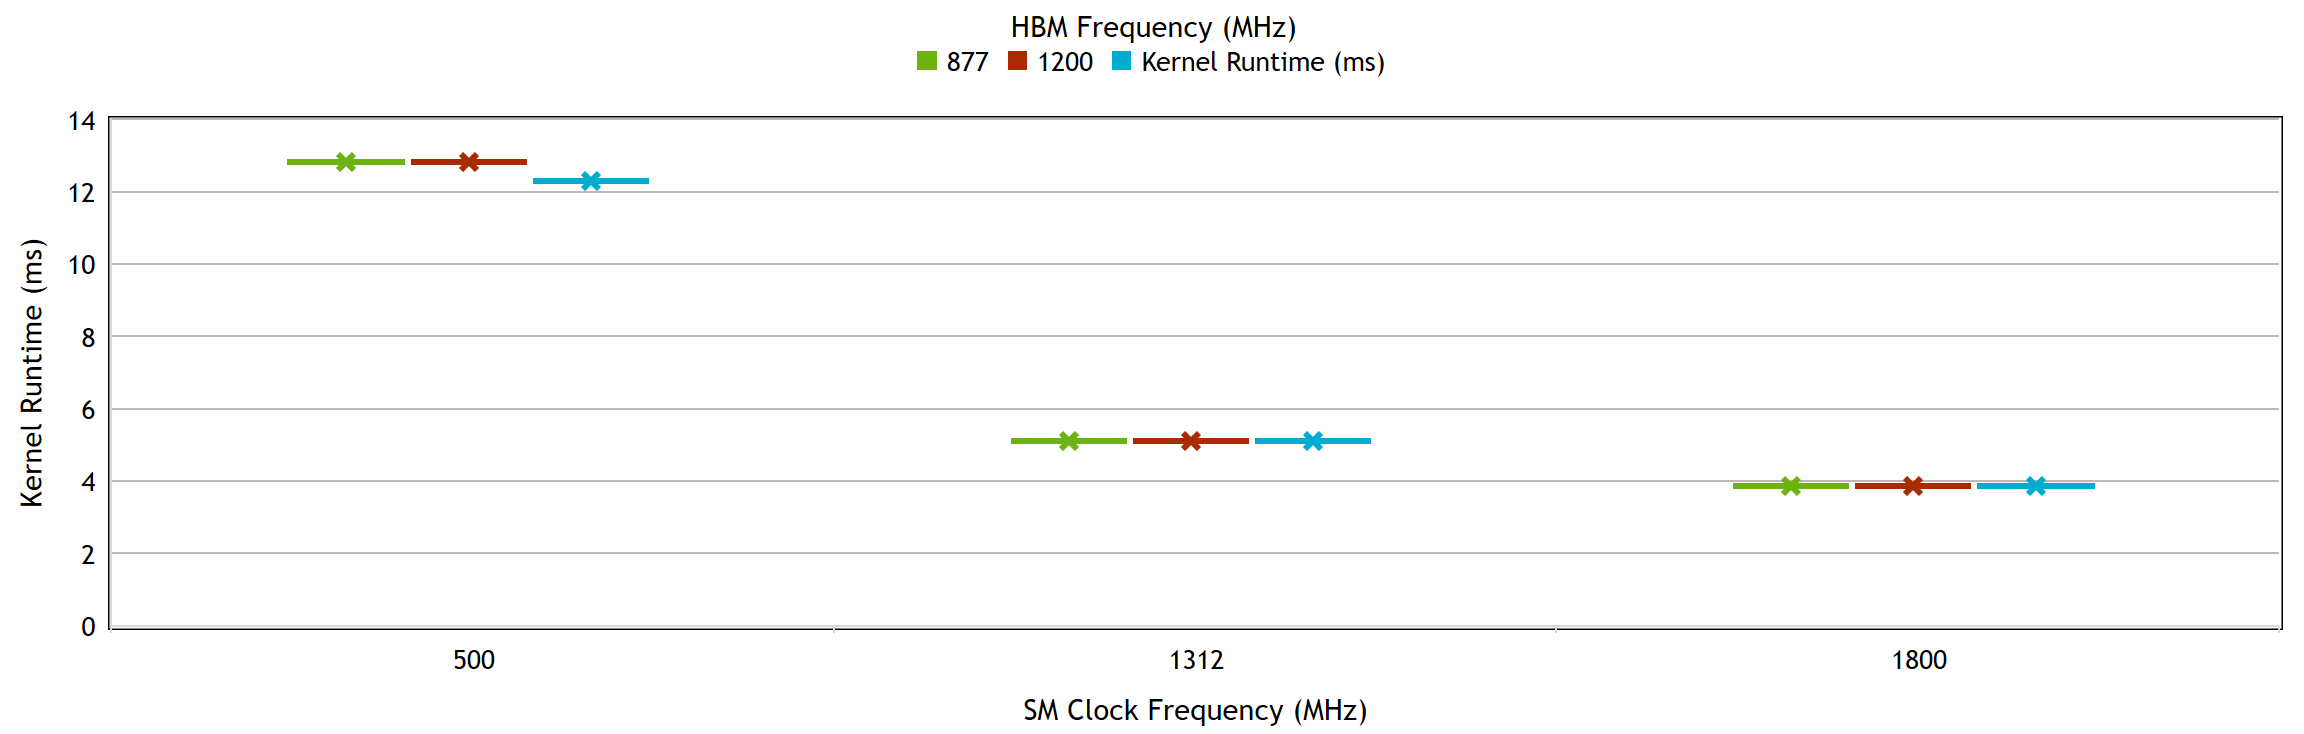
\includegraphics[width=.98\textwidth,keepaspectratio]{figures/lulesh_sweep.png}
      \captionsetup{format=hang, justification=centering, width=.75\textwidth}
      \caption[GPU Parameter Sweep Using LULESH]{GPU Parameter Sweep Using LULESH\\(Baseline was 1312MHz/877MHz)}
      \label{fig:lulesh_sweep}
   \end{figure}


% Design space exploration is not the only use case for this integration. One of
% the more novel features of SST is the ability to obtain periodic statistic dumps
% for all of the currently loaded components. This presents enormous opportunities
% for system designers and application developers. Modern performance profiling
% tools can only provide users with, relatively, coarse-grain details from
% performance counters. SST can provide statistics for any component in the model
% at a time granularity defined by the user. The plots in the figures below are
% all at a 2us granularity. Imagine being able to query that information on any
% time scale for any of the ~20k component statistics in this model! Figure
% \ref{fig:time_sweep} shows an example of this with the host activity plotted in
% \ref{fig:host_cycles} and the GPU crossbar activity plotted in
% \ref{fig:crossbar_activity} (used here as a stand-in for GPU activity).
%
% Kernel launches are asynchronous with the host unless explicitly declared otherwise.
% Even memory copies from the host to the device are asynchronous in this model -- the
% scheduling unit queues all work from a given stream and can guarantee correctness.
%
%    \begin{figure}[!htb]
%       \centering
%       \setlength{\abovecaptionskip}{6pt plus 1pt minus 1pt}
%       \subfigure[Host Cycles]{
%          \label{fig:host_cycles}
%          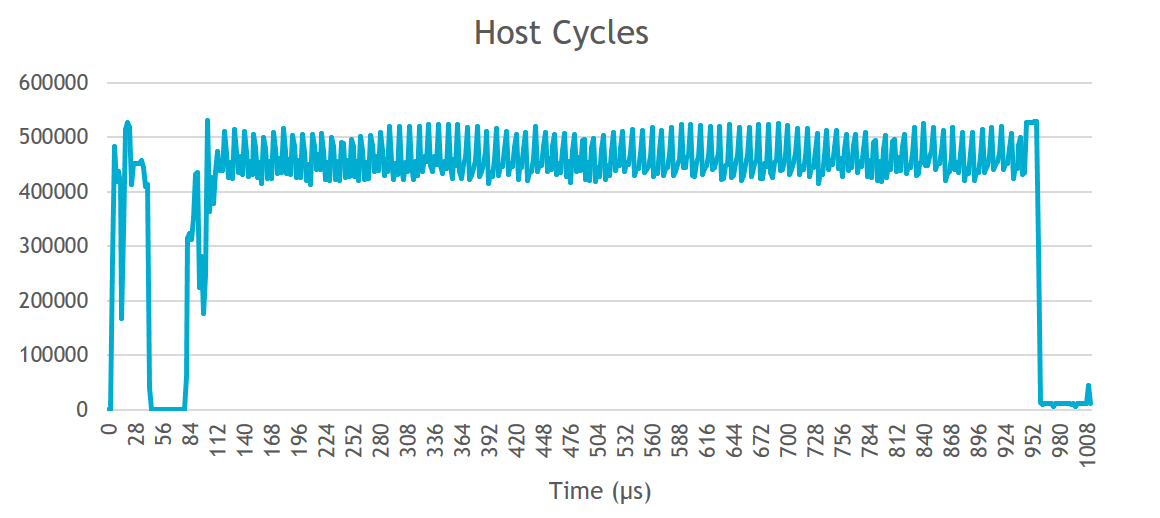
\includegraphics[width=.48\textwidth,height=4cm]{figures/host_cycles.png}
%       }
%       \subfigure[Device Crossbar Activity]{
%          \label{fig:crossbar_activity}
%          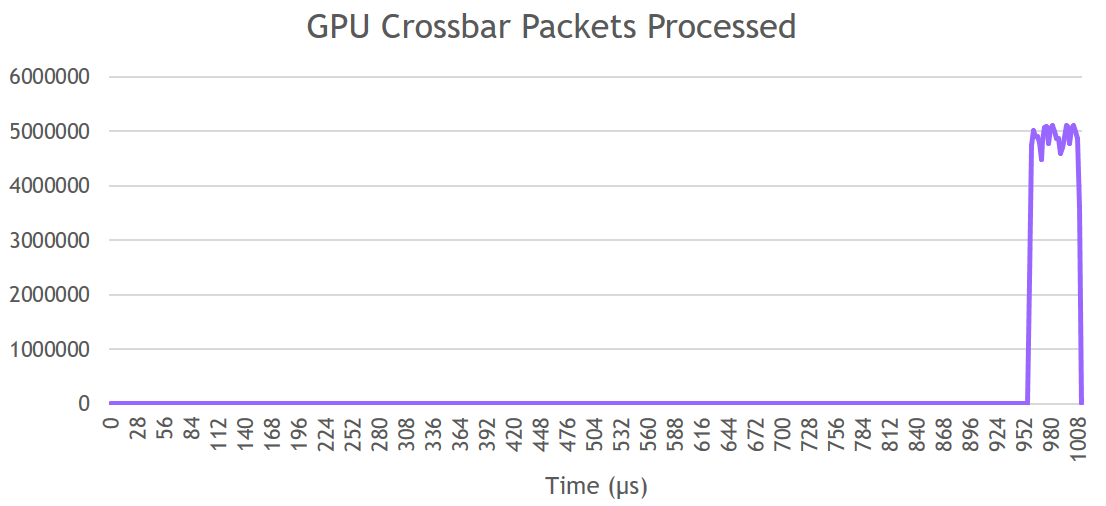
\includegraphics[width=.48\textwidth,height=4cm]{figures/crossbar_packets.png}
%       }
%       \caption{Full caption.}
%       \label{fig:time_sweep}
%    \end{figure}
